\chapter{Ancestral sequence reconstruction of the B cell receptor phylogeny}

\section{Introduction}
With the wide availability and cost reductions of high throughput sequencing (HTS) it is getting commonly applied for studying the immune response through sequencing of the BCR and TCR repertoire.
Phylogenetic reconstruction of the evolution of the BCRs have recently gotten increasing attention because of its possible use in studying vaccine response.
There is a hope that with better understanding of the evolutionary trajectories of BCRs that the fate of the immune response can be modelled in a probabilistic framework, and that this will lead to new avenues in vaccine design finally addressing vaccination of HIV and broad influenza immunity.

By large the use of phylogenetics in BCR GC evolution has been made with the standard assumptions of site independence, constant mutation rates etc. using methods like maximum parsimony \cite{tas2016visualizing}, \cite{Barak2008-fw} and maximum likelihood \cite{Doria-Rose2014-vi}, \cite{Hoehn2016-wg}.
However we find that no study has yet investigated the validity of the phylogenetic assumptions in the context of BCR evolution.
It is important to note that most algorithms for phylogenetic inference have been made to study population genetics largely evolving under a neutrality or track the evolution of organisms over millions of years.
The consequences being that model assumptions are adjusted and validated in a completely different context than the highly selective, small population evolution that BCRs undergo in the GC reaction.
In contrast, BCR evolution has some interesting features that violates the assumption of classical phylogenetic methods e.g. the mutation model is DNA context sensitive, the root of the tree is known, high selection pressure on selected sites, sampled ancestors, very high mutation rates etc.

Validation studies are needed in order to understand weaknesses in the existing phylogenetic tool-chain, and opportunities to develop tools specific to the BCR case.
Sequence simulation is the cornerstone of all validation studies but unfortunately there has been no publicly available method for simulation of BCR sequence evolution.
Multiple articles have described simulations of VDJ recombined sequences \cite{safonova2015igsimulator}, \cite{ralph2016likelihood}, \cite{russ2015htjoinsolver} and few have also described simulation of B cell maturation \cite{shlomchik1998clone}, \cite{kleinstein2003estimating}.
Recombination centric simulations are usually not using a realistic model for simulating the SHM induced mutations in the GC reaction because their purpose is to test VDJ inference, and the few simulation programs emulating maturation are either closed source, does not model central parts of the GC reaction or entirely avoids dealing with sequences.
We are using a branching process, with and without selection, that is developed specifically for modelling the outcome of SHM in the GC reaction to test BCR lineage tree reconstruction under complex evolution.

In this paper we benchmark the performance of classical phylogenetic tools when applied to B cell receptor sequences, including tools for phylogenetic tree inference and for ancestral sequence reconstruction (ASR).
We do so in a realistic sequence simulation framework that can be used in the future for validating BCR specific methods as they develop.




\subsection{Ancestral sequence reconstruction}
When a phylogeny is inferred using a tree as a model for evolution, the tree will have internal nodes connecting the observations.
An internal state is also the inferred common ancestor of a number of leaves and/or branches and therefore sometimes referred to as an ancestral state.
All internal nodes are unknown, unobserved states, either explicitly defined by a sequence as in a parsimony tree, or defined by a likelihood function in model based phylogenies.
When a likelihood function is used to define internal states there is no longer a well defined ancestral sequence, instead this needs to be inferred as the maximum likelihood (ML) sequence estimate.
The ML estimate can be defined in two ways, as either marginal -or joint ML reconstruction.

In a marginal reconstruction the ML estimated sequence for one node is independent of the estimate of another i.e. $a_1 = \operatorname{max}(l(a_1 | t)), a_2 = \operatorname{max}(l(a_2 | t)), \hdots, a_n = \operatorname{max}(l(a_n | t))$, where $l$ is the likelihood function given a tree with branch length and data, $t$, and $a_i$ is an ancestral sequence on internal node $i$.
This makes it easy to find ancestral sequences by iterating through all internal nodes in arbitrary order.

Once an ancestral sequence has been fixed to an internal node this changes the likelihood function for the rest of the tree.
In fact all internal states are interdependent and while this is ignored in the marginal reconstruction it is taken into account in joint reconstruction by maximizing the likelihood of all ancestral states at once i.e. $a_1, a_2, \hdots, a_n = \operatorname{max}(l(a_1, a_2, \hdots, a_n | t)), a_2$.
It is a non trivial task to minimize this likelihood for many internal nodes, and though Pupko et al. \cite{pupko2000fast} showed how to speed up the joint reconstruction algorithm, most software is using the more simple marginal reconstruction.

While it is clear that joint reconstruction is the more probabilistically correct way of inferring ancestral sequences there is less clarity about whether or not this changes the estimated sequences.
The model based methods tested in this work are all using marginal reconstruction and therefore this will also be used in our validation.






\section{Methods}

\subsection{Measuring correctness of ancestral reconstruction}
In the following section we will introduce a benchmark metric for ancestral sequence reconstruction, we call this metric correctness of ancestral reconstruction (COAR).
The correctness of a reconstruction compared to the true evolutionary history can be measured by multiple similarity measures e.g. a) topological similarity, b) branch length similarity and c) sequence similarity between inferred and real ancestors.
All these measures are inter-dependent e.g. the inferred sequences are affected by the branch lengths and the topology and the branch lengths are determined given a topology etc.

Assume the loss function for ancestral sequence reconstruction is comprised of the three above mentioned terms.
The tree topology is the model of the phylogeny by which we can extract useful information like relatedness, ancestral sequences, distances and more.
%EM this next sentence seems strange to me.
Using a wrong topology will therefore be detrimental to the correctness of the phylogeny and likewise the inferred ancestral sequences.
%%% By branch length I also mean the distance from a node to the root
%EM perhaps define branch lengths (expected number of substitutions per site)
Branch lengths are mostly important, in terms of interpretation, if the model underlying the phylogeny is a clock-model.
If a clock-model is not used the interpretation of the branch lengths can be more difficult, but regardless of their magnitude, the branch lengths are merely numbers adjusted by the underlying phylogenetic model, and therefore the correctness of these are of secondary importance.
Lastly, the actual inferred ancestral sequences are determined by a combination of the underlying model, the chosen tree and its branch lengths.
%EM I suggest removing this sentence:
Therefore if the inferred ancestral sequences are correct this gives strong indications about the correctness of both tree topology and branch lengths.
From another perspective the correctness of the inferred ancestral sequences are also the foremost important objective of an ancestral sequence reconstruction when these sequences are used for real applications involving DNA synthesis, protein expression and lab tests.
For these reasons the sole purpose of the COAR metric is to capture the correctness of the inferred ancestral sequences.

%EM I suggest reorganizing this paragraph in such a way that the definition is clear and concise. For example, we hear about gap penalties before we even know what our objective function is.
%EM You could start by describing why we are especially interested in comparing reconstructions from leaf to root, perhaps introducing the ancestral lineage, then note that these lineages can be of different lengths, making comparison non-obvious. The solution is COAR, defined as follows.
%EM fig:ASR_true_vs_inferred is a great figure for motivating COAR.
To calculate the COAR metric two lists of ancestral sequences are compared.
The lists are the ancestral sequences of all the nodes in the direct path going from a leaf to the root.
This is extracted by starting at a leaf node and traversing upwards in the tree, parent by parent, until the root is reached.
In the following, this list of sequences will be referred to as the ancestral lineage.
Two such lists are made, one for the true -and one for the inferred tree, and it is the similarity of these two lists which is the core of the COAR metric.
For lists of similar length the list comparison is easy, it will simply be the cumulated distance between the elements in the two list at the same position e.g. compare list 1 element 1 with list 2 element 1 and list 1 element 2 with list 2 element 2 etc.
This corresponds to the sum of hamming distances between inferred and true ancestors.
However complications arise when the lengths of the lists are not the same which can happen in the case of a wrong topology.
To make a fair comparison between the true -and inferred tree we therefore need to align the two lists and introduce a missing state, called a gap, into one of the lists.
The optimal solution to this alignment problem was described and solved by Needleman and Wunsch \cite{needleman1970general}.
%%% Only if the root is known.
% But also for inferred roots because this has been inferred as the oldest state. OBS: does not apply for some twisted examples:
%T L*****     ***r
%I L*****r
% *is a branching point or cell
We restrict the global alignment result so that it has to start at the root of the tree and end at the leaf sequence because these two states are known, or explicitly inferred, for both the true and inferred phylogenies.
%We restrict the global alignment result so that it has to end at the leaf sequence because this state is known for both the true and inferred phylogenies.
%In the case of phylogenies with known root sequences, e.g. B cell clonal families, there are two known states and therefore another restriction on the alignment.
%EM I think you are saying in this sentence that we further restrict the N-W algorithm to ...
A further restriction on the standard Needleman-Wunsch algorithm is that gaps are only allowed to be introduced in the shortest of the two lists being aligned.
%EM Could you be a little more specific about "undermined"?
The reasoning behind this is that gaps are just a tool to make the most favorable comparison between ancestral lineages, and by introducing gaps in both lists the purpose of comparing sequences is undermined.
With this restriction on gaps, the number of gaps is determined solely by the differences in list lengths and as long as the gap penalty is less than or equal to zero the gaps will always be at the same positions.
Practically this means that the magnitude of the gap penalty only serves the purpose of introducing an extra penalty for inferring a wrong topology and can be adjusted to put more, or less, emphasis on tree topological correctness.
A larger gap penalty meaning more emphasis on correctness of tree topology and vice versa.

One interpretation of the COAR value is that it is the distance between the true -and inferred mutation processes as shown in figure \ref{fig:mutation_process}.
%EM in what sense is it continuous?
With two fixed points, the root and the leaf, whatever is in between, is a continuous mutation process with realizations along this path.
%EM Not sure what this next sentence means.
Realizations in the true tree is a cell division and while it is a branching point on the inferred tree.
The COAR value is then a similarity measure between the realizations of the two mutation processes and in case of missing realizations this will turn into an alignment gap.
In this view more sequences in the inferred ancestral lineage means more realization along the mutational path and vice versa.
The important point being that that those extra realizations could in fact be correctly inferred sequences with no observations in the true phylogeny.
For this reason the gap penalty is chosen to be zero so that the COAR value will only reflect the difference in ancestral lineages and not try to address the possible differences in tree topology.
The correctness of the tree topology can the be assessed separately by other metrics e.g. Robinson-Foulds distance.
\begin{figure}[ht!]
    \centering
    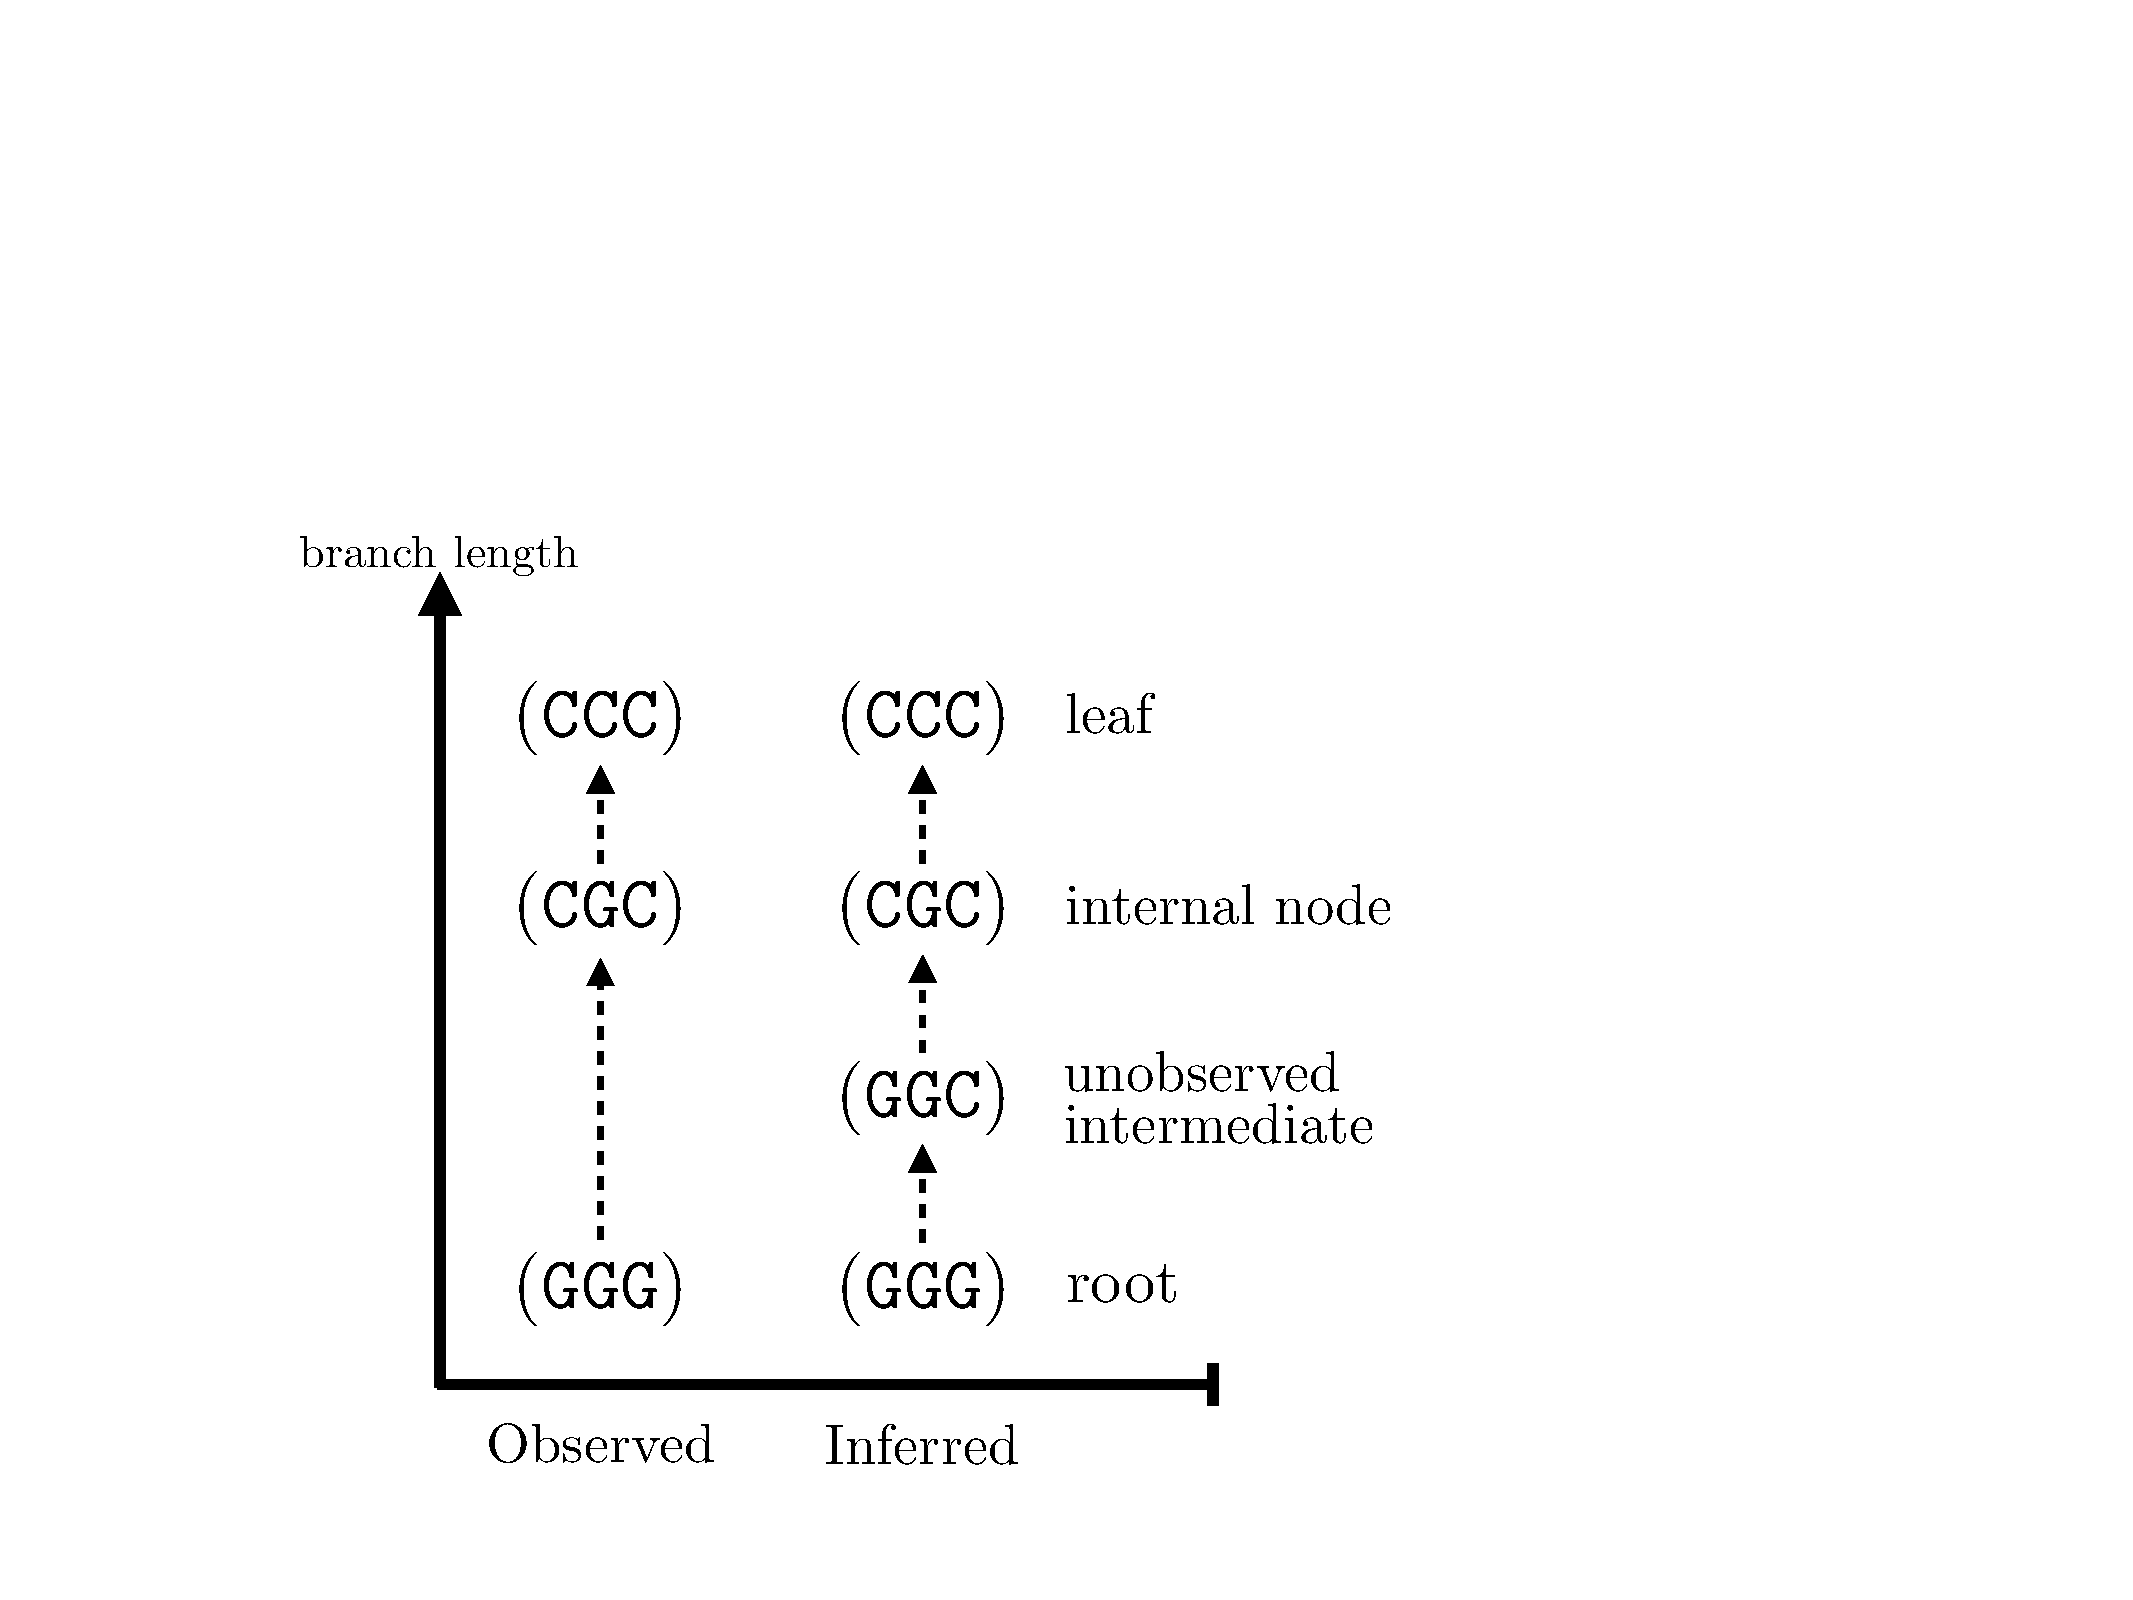
\includegraphics[width=0.5\textwidth]{figures/mutation_process2.pdf}
    \caption{
        \label{fig:mutation_process}
        One interpretation of the COAR value is that it is the distance between the true -and inferred mutation processes, here shown by the true -and inferred ancestral lineage nodes of an example phylogeny. The true ancestral lineage, left side, represents actual observed cells where the genotype is a known constant. The inferred ancestral lineage, right side, represents the estimated genotypes at branching points along the inferred topology. In some cases there is a mis-correspondence between observed cells in the true phylogeny and the branching points in the inferred tree. These are treated as missing realizations and ignored in the alignment of the two mutation processes.
    }
\end{figure}





%%% For phylogenies with known roots
%The ordered list of sequences constitute the reconstructed ancestral lineage for the leaves picked and it always start with the root sequence and ends with the leaf.
% The both the true -and inferred tree may have any number of sequences in this list however there must be as minimum 2; the root and the leaf.


Using the aligned ancestral lineages it is now possible to derive a score, similar to a sequence alignment score, and then normalizing the alignment score to the smallest possible alignment score will give our measure for correctness of ancestral reconstruction (COAR).
$$
\COAR_i = \frac{\alignscore(\leaf_i)}{\alignscore_{\min}(\leaf_i)}
$$
Where alignscore is the score of the alignment between the true and inferred ancestral lineages and in the denominator, $\alignscore_{min}$, is the smallest possible score given the number of sequences in the ancestral lineages.
The alignment score is defined in terms of penalties, so all values are negative, $\alignscore \leq 0$.
Likewise the smallest possible alignment score is negative thereby canceling out the negatives to make a positive COAR.

COAR is defined in the range from 0 to 1, where 0 is a perfect ancestral sequence reconstruction and 1 is the worst possible.
The COAR value is comparable across different trees, methods and datasets because of this normalization, and if the score is proportional to the sequence distance, COAR can be interpreted directly as the average per site error in the inferred ancestral lineage sequences.
%EM This definition more heavily weights the nodes close to the root-- is this an advantage?
COAR for a single ancestral lineage can be expanded to the tree level by calculating the mean COAR value for the whole tree:
$$
\operatorname{mean}(\COAR) = \sum^{L_N}_{i=1} \frac{\alignscore(\leaf_i)}{\alignscore_{\min}(\leaf_i)} / L_N
$$
Where $L_N$ is the number of leaves on the tree.




\subsubsection{Calculating COAR values - example with a known root}
As an example of how the COAR metric works we will present a small example, summarized in figure \ref{fig:ASR_true_vs_inferred} with the light blue leaf chosen for lineage reconstruction and the true and inferred ancestral lineages marked in each tree with red dashed lines.
The example is on the phylogeny of a B cell receptor (BCR) clonal family in which case the root sequence is a known state called the naive sequence.
Assume that the true phylogeny is known with corresponding ancestral sequences along the tree.
Given the leaves of this tree and their sequences a phylogeny can be inferred using any method e.g. maximum parsimony, maximum likelihood, Bayesian methods etc.
We make the restriction that only one inferred tree can be evaluated i.e. if multiple equally parsimonious trees exists one should be chosen at random, or using prior expectations, and if a Bayesian method is used the maximum posterior tree or a random tree weighted according to the posterior distribution should be chosen.
% The true tree will often be derived from simulations while the inferred tree can be made by many different tree algorithms nevertheless these are the basic input to determine the COAR.

\begin{figure}[ht!]
    \centering
    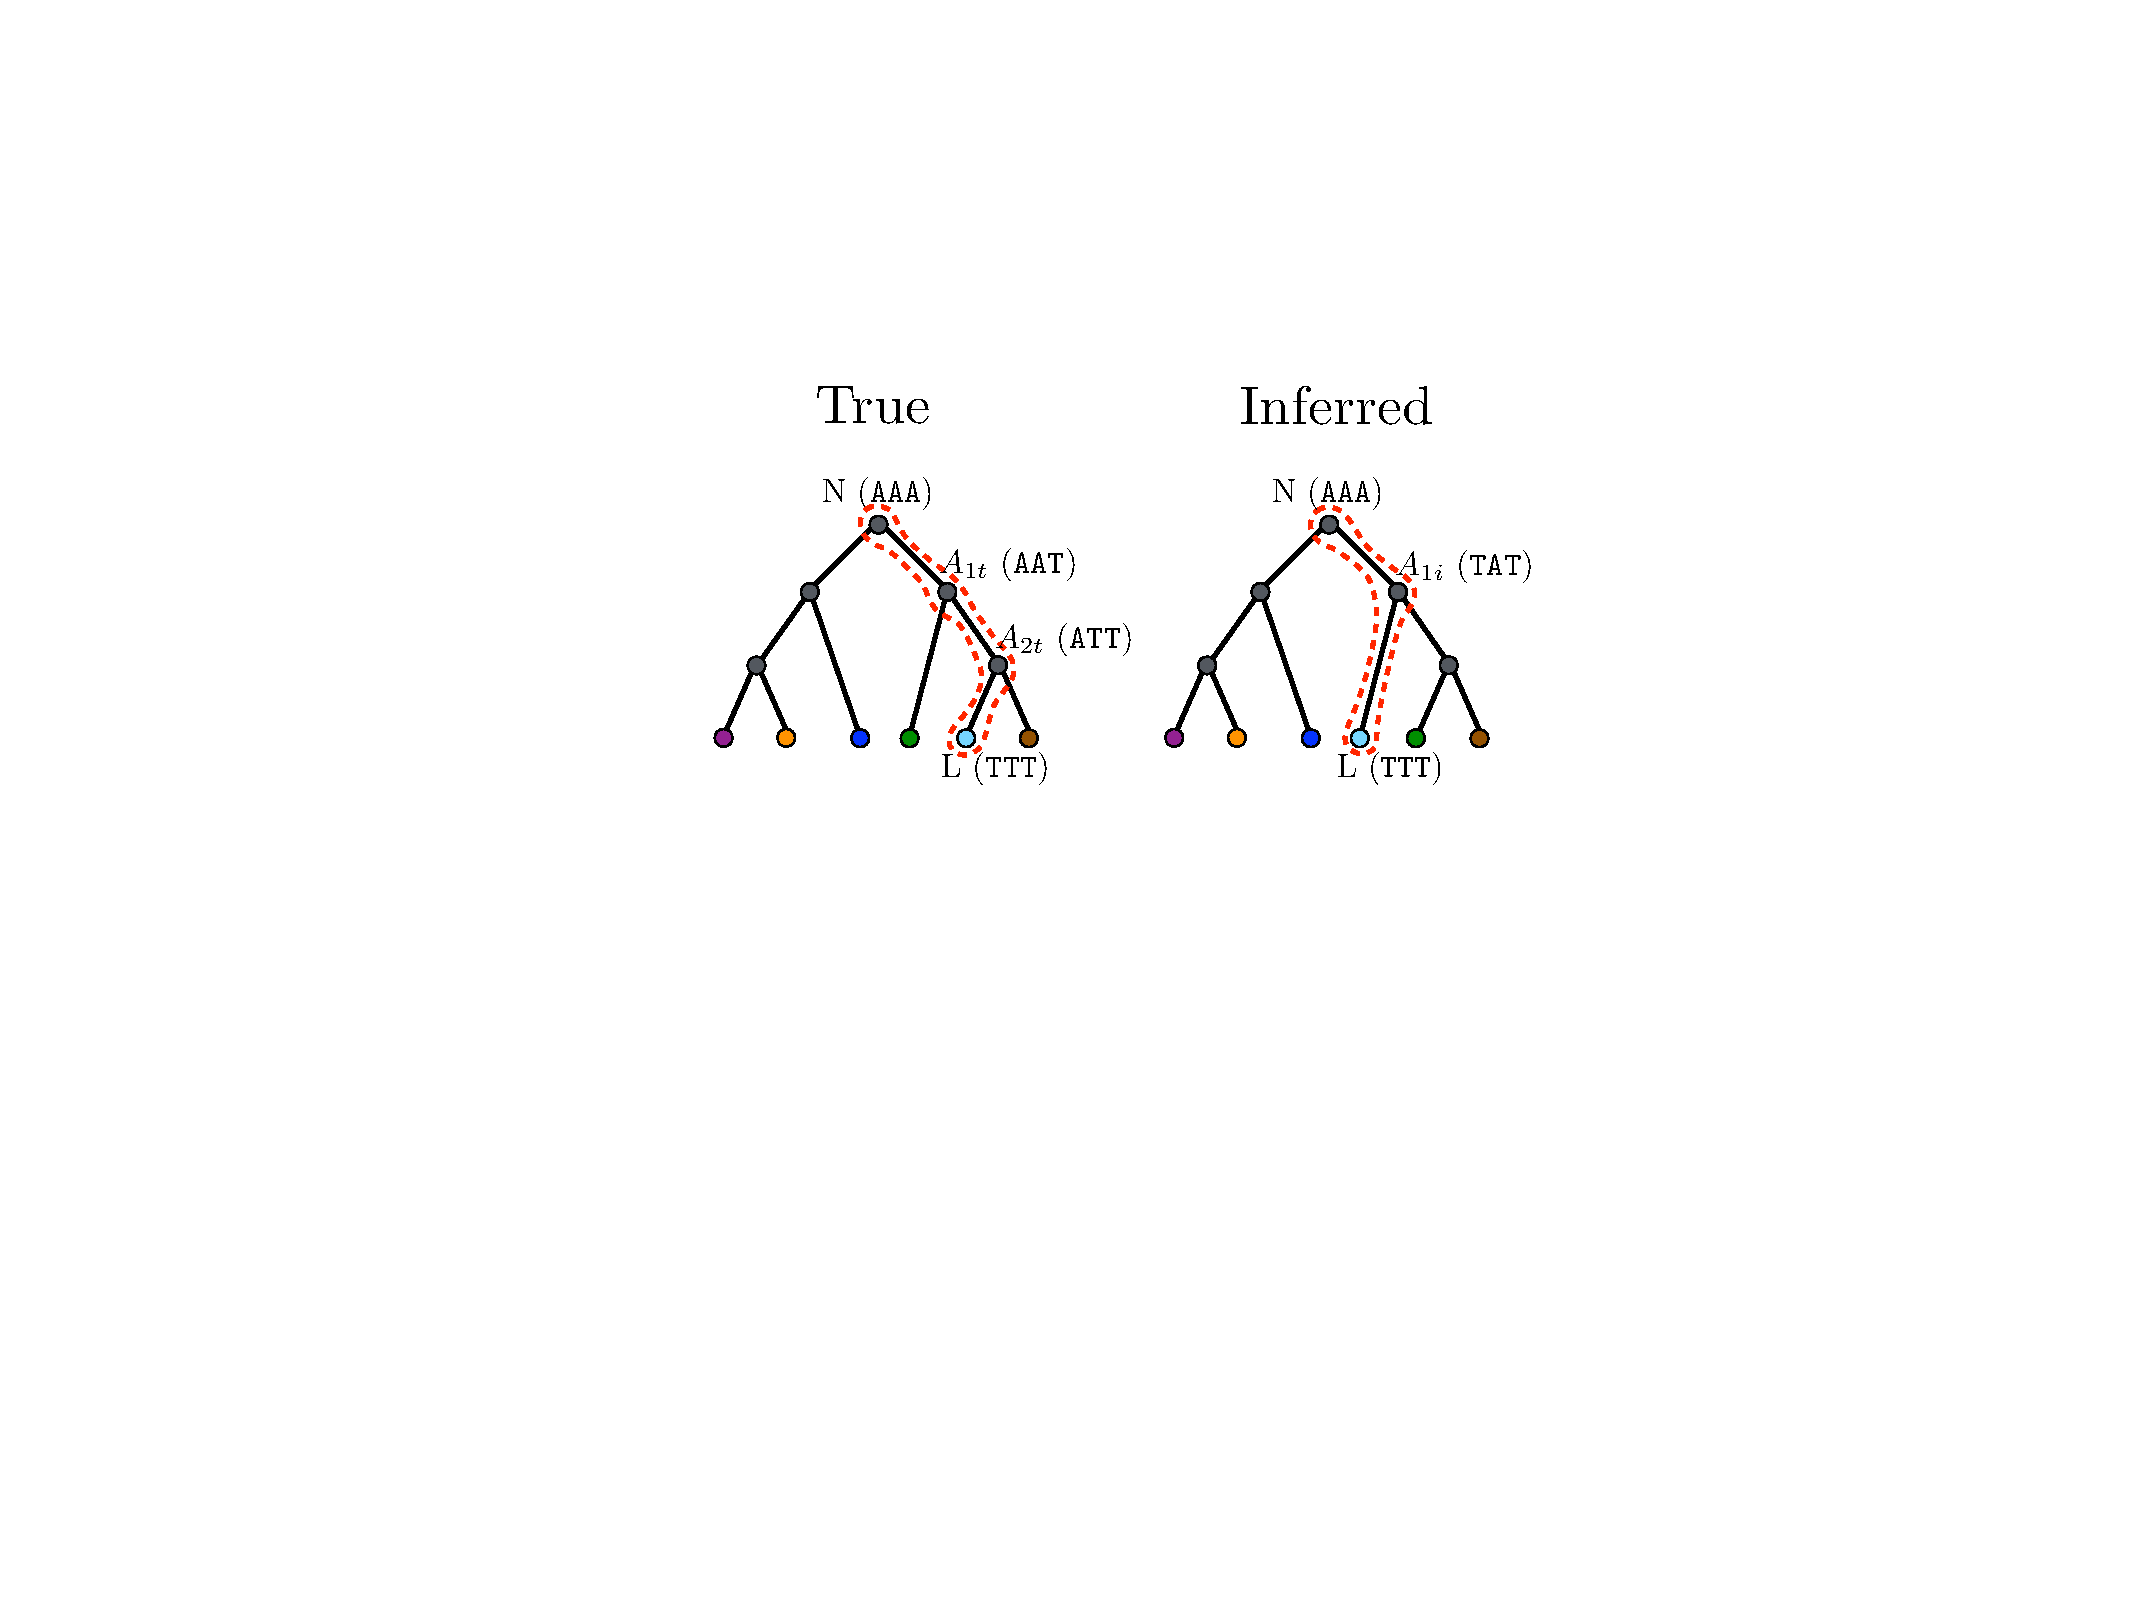
\includegraphics[width=0.7\textwidth]{figures/ASR_true_vs_inferred.pdf}
    \caption{
        \label{fig:ASR_true_vs_inferred}
        True vs.\ inferred tree with colored leaves and grey ancestral states. Reconstruction from the light blue leaf is marked by a dashed red line and annotated with genotypes in parenthesis. N is the naive sequence, L is the leaf sequence and the As are ancestors $1,2,...,n$ with either true or inferred marked by $t$ or $i$, respectively, appended to the subscript. The inferred tree has misplaced the branch leading to the light blue node, resulting in a missing ancestor sequence. The missing ancestor is treated as a missing realization in the inferred mutation process.
    }
\end{figure}

Now take a leaf sequence on the tree and reconstruct its ancestral lineage by extracting the parent, the parent's parent, etc. until the root is reached.
Results for the trees in figure \ref{fig:ASR_true_vs_inferred} are tabulated in table \ref{true_vs_inferred_table}.
This ordered list of sequences constitute the reconstructed ancestral lineage for the chosen leaf and it always start at the root and ends with the leaf sequence.
Both the true -and inferred tree may have any number of sequences in this list, however there must be as minimum 2, the root and the leaf.
In this example the root state is known to be the naive BCR sequence, so we are imposing the restriction on the alignment that it must start with the root and end at the leaf, and that these are known states not counting towards the COAR value.

%Erick stopped here

\begin{table}[ht!]
\centering
\begin{tabular}{rcc}
\multicolumn{1}{c}{} & True   & Inferred \\ \hline
Naive (N)            & \texttt{AAA} & \texttt{AAA}         \\ \hline
$A_1$                & \texttt{AAT} & \texttt{TAT}         \\ \hline
$A_2$                & \texttt{ATT} & -                    \\ \hline
Leaf (L)             & \texttt{TTT} & \texttt{TTT}         \\ \hline
\end{tabular}
    \caption{
         \label{true_vs_inferred_table}
             Reconstructed ancestral lineage for true -and inferred trees as shown in figure \ref{fig:ASR_true_vs_inferred}.
             }
\end{table}

%%%% Maybe include abundances in the example later:
\iffalse

\begin{table}[ht!]
\centering
\label{table:true_vs_inferred_table}
\begin{tabular}{rccc}
\multicolumn{1}{c}{} & True   & Inferred & Abundance \\ \hline
Naive (N)            & \texttt{AAA} & \texttt{AAA}   & 1         \\ \hline
$A_1$                & \texttt{AAT} & \texttt{AAT}   & 2         \\ \hline
$A_2$                & \texttt{ATT} &                  & 20        \\ \hline
Leaf (L)             & \texttt{TTT} & \texttt{TTT}   & 5         \\ \hline
\end{tabular}
\end{table}

\fi

%To align the true vs.\ inferred lists of reconstructed ancestral lineages we will consider each sequence as a state that can be compared to another state to find

In cases of a wrongly inferred topology the true and inferred lists of ancestral lineage sequences can have different lengths, so we need a way of finding the best possible alignment between these lists.
We know the start and end of this alignment since that is defined as the shared root and leaf sequences, but the sequences between are free to be shifted up or down to maximize the alignment fit.
This problem is similar to that of the global sequence alignment problem solved by Needleman and Wunsch \cite{needleman1970general}.
The solution can be implemented by dynamic programming and solved in squared time complexity.
In this example phylogeny the calculation will be explicitly state by showing the matrix operations, but these operations also applies in the general case of the algorithm.
A notable difference to the original Needleman-Wunsch algorithm is that it was intended to align two sequences of characters, like DNA or amino acids, while in this application instead of aligning a list of sequence characters a list of whole sequences are aligned.

% The first step in the alignment algorithm is to calculate a distance matrix of all pairwise distances.
The first step in the alignment algorithm is to calculate a score matrix of all pairwise sequence comparisons.
For this example we use the negative of the distance between sequences as a score and therefore populating the score matrix is a simple procedure of calculating hamming distances.
However the score function can be extended to reflect different situations, like larger penalty for non-synonymous rather than synonymous mutations.
By using simple hamming distances, we will in this example be weighting all mismatches equally.
The score matrix is tabulated in table \ref{distance_matrix}.
We use negative scores to reflect that mismatches represents a loss.
% This matrix is called the score matrix to stress the fact that it is not exclusively for string distances but can accommodate more advanced loss functions.

\begin{table}[ht!]
\centering
\begin{tabular}{c|r|r|r|r}
\rowcolor[HTML]{EFEFEF}
                                 & \multicolumn{1}{c|}{\cellcolor[HTML]{EFEFEF}N} & \multicolumn{1}{c|}{\cellcolor[HTML]{EFEFEF}$A_{1t}$} & \multicolumn{1}{c|}{\cellcolor[HTML]{EFEFEF}$A_{2t}$} & \multicolumn{1}{c}{\cellcolor[HTML]{EFEFEF}L} \\ \hline
\cellcolor[HTML]{EFEFEF}N        & 0                                              & -1                                                    & -2                                                    & \multicolumn{1}{r|}{-3}                       \\ \hline
\cellcolor[HTML]{EFEFEF}$A_{1i}$ & -2                                             & -1                                                     & -2                                                    & \multicolumn{1}{r|}{-1}                       \\ \hline
\cellcolor[HTML]{EFEFEF}L        & -3                                             & -2                                                    & -1                                                    & \multicolumn{1}{r|}{0}                        \\ \hline
\end{tabular}
    \caption{
         \label{distance_matrix}
             Score matrix based on all pairwise distances between the sequence in figure \ref{fig:ASR_true_vs_inferred}.
             }
\end{table}

% To allow for different lengths of true and inferred list of ancestral sequences they are align with the possibility of a gap to be introduced.
% This gap should be penalized to reflect the difference between true and inferred ancestral lineages.
%%% Next line is true only because the gap penalty is influencing the maximum penalty and thereby shifting the COAR. It will never influence the actual alignment.
%%%%%%% This depends or whether a restriction is put on the gap introduction. E.g.\ this could be allowed:
% AA-AAA
% BBB-BB
% The magnitude of the gap penalty is determined to put appropriate amount of emphasis on correctness of the tree topology.
% In this example we will use a hard penalty on wrong topology by setting the gap penalty to -10.
% In a realistic setting the gap penalty should depend on the length of the sequences on the input tree and e.g. a gap penalty of 10\% of the sequence length would be sufficient to penalize wrong topologies without over emphasizing the importance compared to similarity in ancestral sequences.
% So in the example of an input tree with sequences of length 300 a gap penalty of -30 would be a good choice.
%It it worth to notice that in this example, because the first and last sequence in the alignment is fixed to the root and leaf, the number of gaps is fixed

Now we are ready to initializing the alignment grid central to the Needleman-Wunsch algorithm.
Initialization is started by inserting the scores of pure gap characters i.e. first row and first column, see table \ref{NW_fill_table1}.
Since the naive sequence is known we require the two root sequences to align by setting this gap penalty to negative infinity.
Similarly we disallow introduction of gaps in the longest of the sequence lists by penalizing these as negative infinity as seen in table \ref{NW_full_table}.
Setting certain gap penalties to negative infinity is a simple way of dealing with disallowed gaps and it works well in an implementation.
\begin{table}[ht!]
\centering
\begin{tabular}{c|r|r|r|r|r|}
\rowcolor[HTML]{EFEFEF}
                                 & \multicolumn{1}{c|}{\cellcolor[HTML]{EFEFEF}-} & \multicolumn{1}{c|}{\cellcolor[HTML]{EFEFEF}N} & \multicolumn{1}{c|}{\cellcolor[HTML]{EFEFEF}$A_{1t}$} & \multicolumn{1}{c|}{\cellcolor[HTML]{EFEFEF}$A_{2t}$} & \multicolumn{1}{c|}{\cellcolor[HTML]{EFEFEF}L} \\ \hline
\cellcolor[HTML]{EFEFEF}-        & 0                                              & -Inf                                            & -Inf                                                   & -Inf                                                   & -Inf                                            \\ \hline
\cellcolor[HTML]{EFEFEF}N        & -Inf                                            & ->                                            &                                                    &                                                    &                                             \\ \hline
\cellcolor[HTML]{EFEFEF}$A_{1i}$ & -Inf                                            &                                             &                                                    &                                                    &                                             \\ \hline
\cellcolor[HTML]{EFEFEF}L        & -Inf                                            &                                             &                                                    &                                                    &                                             \\ \hline
\end{tabular}
    \caption{
         \label{NW_fill_table1}
             The starting alignment grid, initialized with the gap penalties which is negative infinity to disallow gap opening in the beginning of the alignment. The grid is filled up from left to right row by row, starting in the cells with left, top and diagonal cells filled (marked by ->).
             }
\end{table}


Then the alignment grid is filled up starting with the cell that has left, top and diagonal cells filled (marked by -> in table \ref{NW_fill_table1}) and continuing to the right side cell that also has left, top and diagonal cells filled.
Each cell is filled up by the following equation:
$$
C_{i,j} = max\left\{ (C_{i-1,j} + gp_{down}); (C_{i,j-1} + gp_{right}); (C_{i-1,j-1} + SC_{i-1,j-1})  \right\}
$$
Moving in the order $i=1,2,3,4$ and $j=1,2,3,4,5$. Where $C_{i,j}$ is the ith row and jth column cell in the grid, $SC_{i-1,j-1}$ is the score of aligning the ith, jth elements found by look-up in the the score matrix (table \ref{distance_matrix}) and $gp_{down}$ and $gp_{right}$ is the gap penalty of the moving down and right respectively.
In this example the longest sequence list is the true ancestral lineage and therefore gaps are only allowed to be introduced into the inferred list of sequences.
The penalty for introducing gaps in the true list of sequences is set to negative infinity to reflect this and therefore $gp_{down} = -\Inf$ and $gp_{right} = 0$.

The grid is filled and results store in table \ref{NW_full_table}.
The final alignment score is the number in the rightmost bottom cell.
\begin{table}[ht!]
\centering
\begin{tabular}{c|r|r|r|r|r|}
\rowcolor[HTML]{EFEFEF}
                                 & \multicolumn{1}{c|}{\cellcolor[HTML]{EFEFEF}-} & \multicolumn{1}{c|}{\cellcolor[HTML]{EFEFEF}N} & \multicolumn{1}{c|}{\cellcolor[HTML]{EFEFEF}$A_{1t}$} & \multicolumn{1}{c|}{\cellcolor[HTML]{EFEFEF}$A_{2t}$} & \multicolumn{1}{c|}{\cellcolor[HTML]{EFEFEF}L} \\ \hline
\cellcolor[HTML]{EFEFEF}-        & 0                                              & -Inf                                            & -Inf                                                   & -Inf                                                   & -Inf                                            \\ \hline
\cellcolor[HTML]{EFEFEF}N        & -Inf                                            & 0                                              & 0                                                   & 0                                                   & 0                                            \\ \hline
\cellcolor[HTML]{EFEFEF}$A_{1i}$ & -Inf                                            & -Inf                                            & -1                                                     & -1                                                   & -1                                            \\ \hline
\cellcolor[HTML]{EFEFEF}L        & -Inf                                            & -Inf                                            & -Inf                                                   & -2                                                    & -1                                            \\ \hline
\end{tabular}
    \caption{
         \label{NW_full_table}
             The filled alignment grid, ready for tracing back the best alignment. The rightmost bottom cell has the score for the best alignment.
             }
\end{table}

Last step is to traceback the best path through the alignment grid and store this alignment.
The traceback starts from the leaf sequence, in the right bottom corner, and ends with the naive sequence in the left top corner.
A diagonal step is equivalent to a sequence match, a left move is introducing a gap character in the inferred list and a move up is introducing a gap in the true list.
The path is found by moving backwards following the same path that was used to fill up the grid, and therefore using the same equation as to fill it, just reversed with moving from bottom right cell to top left, $i=4,3,2,1$ and $j=5,4,3,2,1$:
%$$
%move_{i,j} = which\left\{ (C_{i-1,j} + gp_{down} = C_{i,j}); (C_{i,j-1} + %gp_{right} = C_{i,j}); (C_{i-1,j-1 } + SC_{i-1,j-1} = C_{i,j})  \right\}
%$$
$$
move_{i,j} = which\left\{ C_{i,j} = [(C_{i-1,j} + gp_{down}), (C_{i,j-1} + gp_{right}), (C_{i-1,j-1 } + SC_{i-1,j-1})] \right\}
$$
Notice that this path has already been generated when the alignment grid was filled up and could be cached. The resulting alignment and the penalty for each position is tabulated in table \ref{NW_final_alignment}.

Lastly this value is normalized by the smallest possibly alignment score assuming that all matched positions contained sequences with maximal distances i.e. no similarity, this normalized number is the COAR values and it runs between 0 to 1.
In the presented example we only calculated the COAR value for the reconstructed ancestral lineage from one leaf node but doing the calculations on all leaves on the tree and taking the average would give the the mean COAR value for the whole tree.
% Doing the same calculations on all leaves on the tree and summing this will give the total alignment score of the inferred phylogeny.
\begin{table}[ht!]
\centering
\begin{tabular}{|lcccc|}
\hline
\multicolumn{1}{|l|}{True}     & \multicolumn{1}{c|}{N} & \multicolumn{1}{c|}{$A_{1t}$} & \multicolumn{1}{c|}{$A_{2t}$} & T                      \\
\multicolumn{1}{|l|}{Inferred} & \multicolumn{1}{c|}{N} & \multicolumn{1}{c|}{$A_{1i}$} & \multicolumn{1}{c|}{-}        & T                      \\ \hline
Penalty                        & 0                      & -1                             & 0                           & 0                      \\ \hline
Max penalty                    & \multicolumn{1}{l}{0}  & \multicolumn{1}{l}{-3}        & \multicolumn{1}{l}{0}       & \multicolumn{1}{l|}{0} \\ \hline
COAR                           & \multicolumn{4}{c|}{-1/-3=0.333}                                                                                    \\ \hline
\end{tabular}
    \caption{
         \label{NW_final_alignment}
             The resulting alignment and the penalty for each positions.
             }
\end{table}





\subsection{Other validation metrics}

\subsubsection{Most recent common ancestor distance}
As an alternative to COAR we are also using a measure named the "most recent common ancestor" (MRCA) metric.
In this more simple measure of correctness of ASR the MRCA ancestral sequence between two leaves are found and compared in the true vs.\ inferred phylogeny.
By iterating through all pairwise combinations of leaves the MRCA distance can be found as the sum:
$$
\MRCA_{\dist} = \sum_{i=1}^{N} \sum_{j=i+1}^{N} \dist(T_{MRCA}(l_i, l_j), I_{MRCA}(l_i, l_j))
$$
All the pairwise combinations of leaves $l_i$ and $l_j$ ($i \neq j$) to find their true ($T_{MRCA}$) -and inferred ($I_{MRCA}$) MRCA.
The distance between the two ancestral sequences are found with the function $\dist(\cdot, \cdot)$ and summed over all pairs.
In this work we use the hamming distance as distance function.

Similar to COAR, ancestral sequences close to the root will have more influence on the result than sequences close to the tips.
The major difference is that MRCA is not scaled and not representing the result of a lineage reconstruction and can therefore the value has no meaningful interpretation aside from measuring performance of different method on identical data.


\subsubsection{Robinson–Foulds distance}
The tree topology is the model that explains the order of branching events and relatedness of leaves, and therefore inferred ancestral sequences will always be tied to the topology.
Hence validating the ASR should also express some degree of correctness of the tree.
Regardless it is interesting to have a method solely expressing the correctness of inferred tree topology so for this purpose we use the Robinson–Foulds (RF) distance \cite{robinson1981comparison}.
Briefly the RF distance is defined as the number of different tree partitions between two trees.
Tree partitions are made by cutting a branch connecting two nodes, all possible cuts are performed and the resulting split of taxa are sorted and recorded into two columns.
The after sorting the list of partitions they are compared true vs.\ inferred tree and for each partition mismatch the RF distance is increased by 1.



\subsection{Algorithms tested}
With the exception of a few methods there has been little published about BCR phylogeny specific software.
Barak et al. made some vaguely defined rules written into a an algorithm they named IgTree \cite{Barak2008-fw}.
The description of IgTree is similar to that of maximum parsimony (MP) and it is unclear whether there is any difference at all.
For that reason we use the MP algorithm \texttt{dnapars} from PHYLIP \cite{plotree1989phylip} as a substitute for IgTree and other methods e.g. Tas et al. \cite{tas2016visualizing}.

In the paper from Doria-Rose et al. \cite{Doria-Rose2014-vi} they use the general time reversible (GTR) model implemented in MEGA5 \cite{tamura2011mega5}.
Similarly Kepler \cite{Kepler2013-sy} was using \texttt{dnaml} from the PHYLIP package to infer BCR phylogenetic trees.
To test these commonly used maximum likelihood trees we use \texttt{dnaml}.

Two different models have been defined specifically for BCR evolution on protein level, the AB amino acid substitution matrix from Mirsky et al. \cite{mirsky2014antibody} and HLP17 codon model from Hoehn et al. \cite{Hoehn2016-wg}.
Both are implemented with codonPhyML \cite{gil2013codonphyml}.
The AB substitution matrix is just a standard amino acids substitution rate matrix but fitted to substitutions observed in BCR sequences, yielding a symmetric rate matrix that assumes equilibrium.
But recently Sheng et al. found large discrepancies between their findings and the AB substitution matrix \cite{sheng2017gene}, promoting us to exclude this from our evaluation.
Instead we test the HLP17 model as it is implemented in the software IgPhyML (\url{github.com/kbhoehn/IgPhyML}).
The HLP17 model is based on a GY94 model \cite{goldman1994codon} but adding parameters to account for AID hot/cold spots and thereby attempting to address the context sensitivity of SHM.

Lastly we also test the performance of an unpublished method that uses a likelihood based ranking of equally parsimonious trees, we call this method GCtree, for genotype collapsed tree.
Briefly, the likelihood function is based on the assumption that the GC reaction can be modelled as a binary Galton-Watson process \cite{harris2002theory}.
Some genotypes have many observations while others have fewer, the Galton-Watson process will favour a high abundance genotype to be the parent for a low abundance genotype.
Each MP tree is evaluated and ranked according to its fit and then the highest likelihood tree is picked out as the GCtree inferred tree.



\subsection{Simulated data}
Simulations were performed using both the neutral branching process and the affinity simulation previously described in chapter 3.
Both simulation, inference and evaluation was wrapped into an SCons script \cite{fomel2007reproducible} available in the codebase of \texttt{GCtree} (\url{github.com/matsengrp/gctree}).
SCons commands used can be found in appendix C.





\section{Results - comparing algorithms for B cell phylogenetic reconstruction}
The most suitable dataset for clonal family phylogeny is dara collected from a single GC like one in Tas et al. \cite{tas2016visualizing}.
But unlike single cell sequences most data is generated from bulk RNA extract from peripheral blood mononuclear cell (PBMC).
To adjust the simulation parameters to recapitulate a given dataset we both used the single cell Tas dataset (see appendix B), and an HTS dataset generated from PBMCs from HIV infected individuals.
In these HTS datasets cluster were done using partis resulting in hundreds of clonal families.
To only isolate HIV relevant clonal families a seed sequence was used and only sequence in the same clonal family was extracted.
Seed sequences were generated by single cell screening of the memory fraction of the PBMCs, followed by Sanger sequencing of the cells expressing HIV neutralizing antibodies.
The size of the clonal families varied substantially as shown in figure \ref{fig:Laura-neutsim_Laura-data}, but they serve as a more realistic dataset case than the single cell data from Tas et al.


Simulation parameters are adjusted in order to recapitulate two measures: a) distribution of sequence across the length of the tree and b) how "spread out" the tree leaves.
Measure a) is captured by plotting the CDF of the distance to the naive/root sequence ((a) in figure \ref{fig:Laura-neutsim_Laura-data} and \ref{fig:Laura-affsim_Laura-data}).
Measure b) is captured by plotting the CDF of the nearest neighbor distance ((b) in figure \ref{fig:Laura-neutsim_Laura-data} and \ref{fig:Laura-affsim_Laura-data}).
The neutral simulation with a high $\lambda$ will naturally vary a lot early population size an therefore had no problem fitting into the large span of possible summary statistics defined by two chosen clonal family representatives from the HTS data, see figure \ref{fig:Laura-neutsim_Laura-data}.
The nature of the affinity simulation forces it to have a rather constant population size defined by its carrying capacity.
Instead the GC was down-sampled to 150 sequence and the variance in the number of observed sequences comes from the fact that some sequences are identical at DNA level and deduplicated, see figure \ref{fig:Laura-affsim_Laura-data}.

\begin{figure}[!ht]
    \begin{center}
    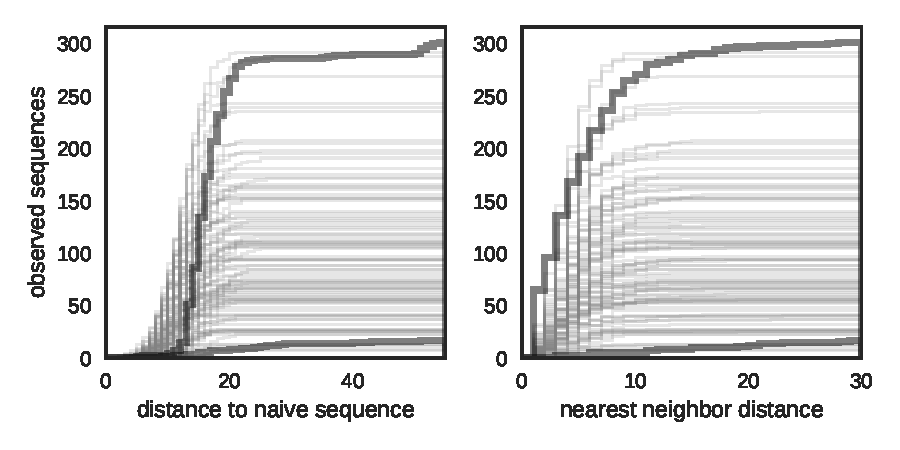
\includegraphics[width=0.8\textwidth]{figures/Laura-neutsim_Laura-data.pdf}\newline%
    \end{center}
    \vspace{-14mm} \hspace{44mm} (a) \hspace{50mm} (b)
    \caption{
        \label{fig:Laura-neutsim_Laura-data}
        Summary statistics for the unique sequences simulated under a neutral model fitted to HTS data.
        The two thick dark grey lines represents the characteristics of two clonal families extracted by partis seed clustering on HTS data.
        Smaller light grey lines are showing 1 of the 100 simulated datasets.
        Non default parameters used: $T=5$, $\lambda=2.5$, $\lambda_0=3$
    }
\end{figure}

\begin{figure}[!ht]
    \begin{center}
    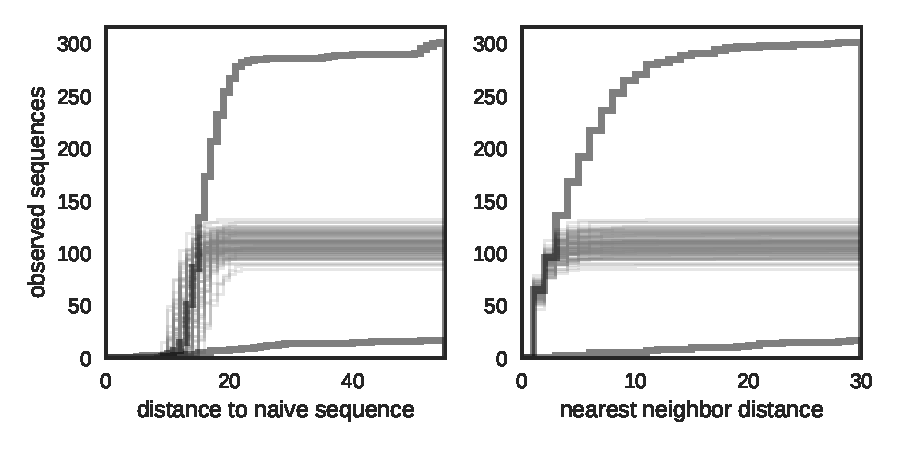
\includegraphics[width=0.8\textwidth]{figures/Laura-affsim_Laura-data.pdf}\newline%
    \end{center}
    \vspace{-14mm} \hspace{44mm} (a) \hspace{50mm} (b)
    \caption{
        \label{fig:Laura-affsim_Laura-data}
        Summary statistics for the unique sequences simulated under the affinity model fitted to HTS data.
        The two thick dark grey lines represents the characteristics of two clonal families extracted by partis seed clustering on HTS data.
        Smaller light grey lines are showing 1 of the 100 simulated datasets.
        Non default parameters used: $T=90$, $n=150$, $\lambda_0=0.25$
    }
\end{figure}


Looking a RF distance for the neutral simulation there are only small differences and only the distribution of RF distances for MP is shift up compared to the others (significant $p<0.05$ in Mann–Whitney U (MWU) test), see figure \ref{fig:Laura-neutsim_valid}.
Likewise the quartiles are slightly shifted upward for MP in the comparison of MRCA distances.
We consider COAR the most important metric because this has a direct interpretation inspired by the purpose of the tree, and for COAR there seems to be no significant difference between the methods when simulating under neutral conditions.
The average COAR values are ranging from 1.76E-04 to 2.37E-04 (appendix A table \ref{tab:Laura-neutsim_vali}) corresponding to approx. 10\% chance of one nucleotide error per reconstructed sequence in a lineage from leaf to root.
Similar but somewhat large differences are observed for neutral simulation using parameters fitted to the Tas dataset, see figure \ref{fig:Tas-neutsim_vali} in appendix B.
Should we rank the methods based on all metrics from best to worst the rank would be: GCtree, dnaml, IgPhyML, Parsimony.
But the first three are virtually the same.
The Tas dataset fitted simulations also experience a similar range of expected errors in ASR, though slightly lower because of the fewer sequences simulated, see table \ref{tab:Tas-neutsim_vali} in appendix A.

\begin{figure}[!ht]
    \centering
    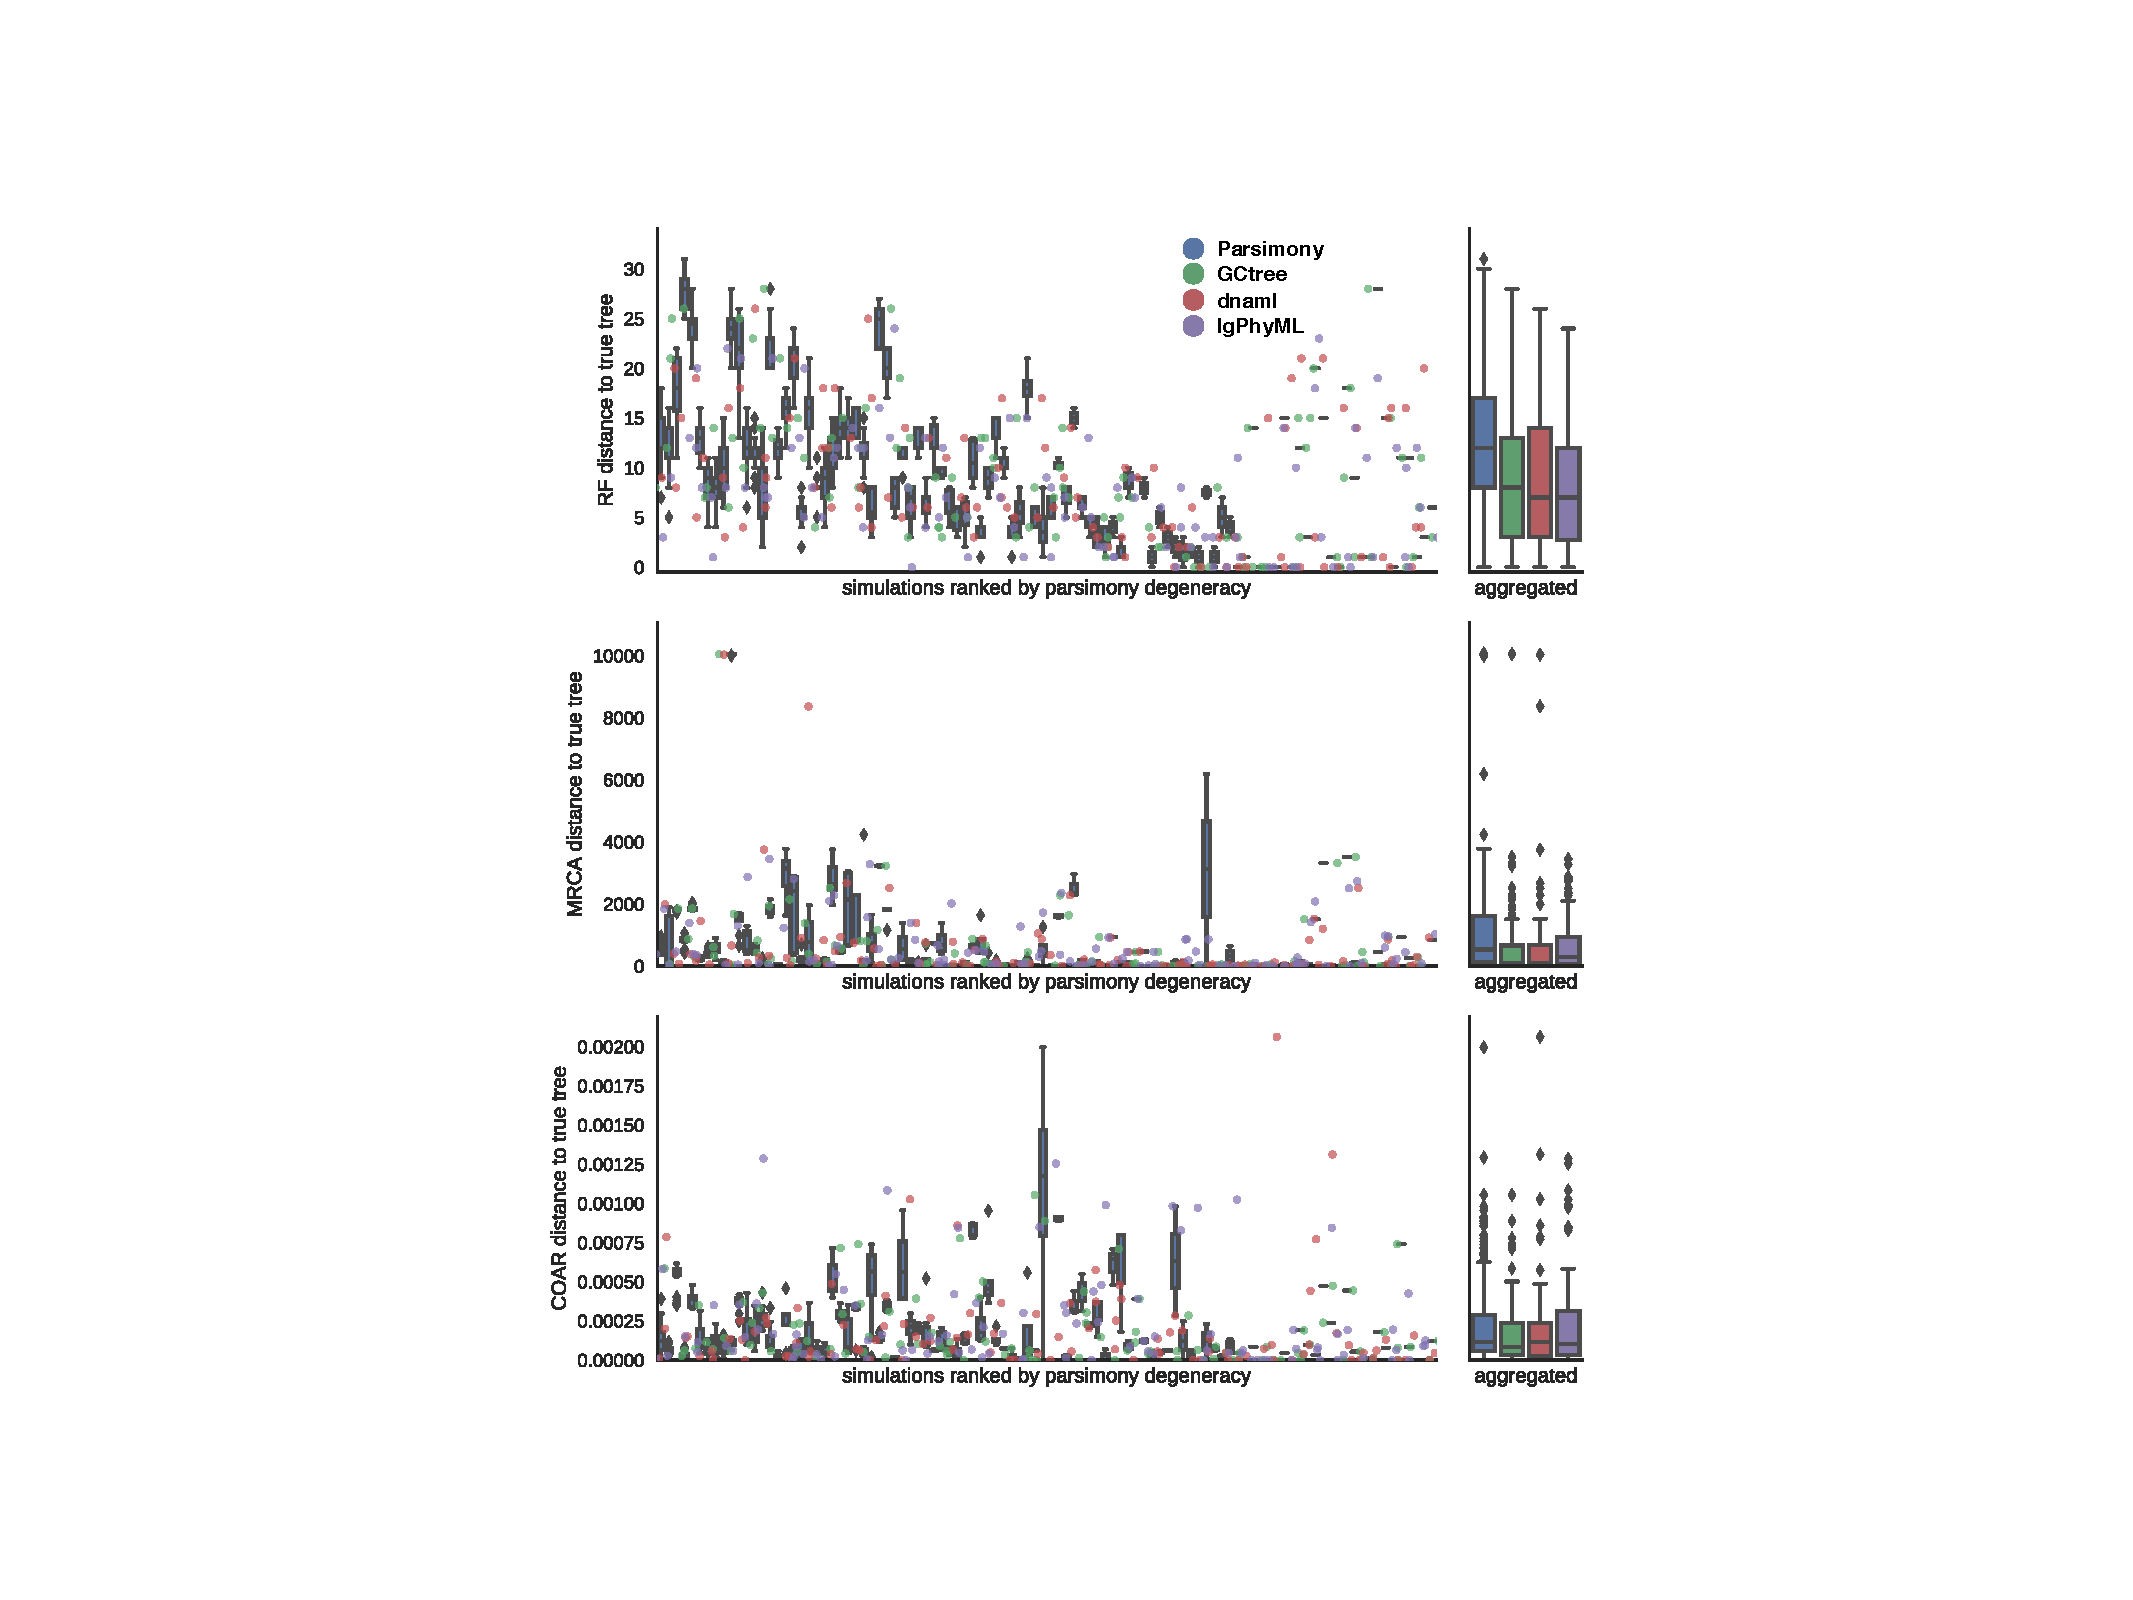
\includegraphics[width=0.9\textwidth]{figures/Laura-neutsim_valid.pdf}
    \caption{
        \label{fig:Laura-neutsim_valid}
        Simulation with 100 repeats of a neutral branching process.
        Each simulation is plotted in a single column ranked according to the number of equally parsimonious trees for the simulation.
        The ensemble of equally parsimonious trees are shown as a box plot while the other methods are plotted as jittered dots.
        On the right the aggregated result is shown.
    }
\end{figure}
\clearpage


For the affinity simulations we allow genotypes to reappear in another clade during simulations i.e. homoplasy is allowed.
This prevents us from calculating the RF distance but not from the other metrics.
However for both MRCA and COAR there is no significant differences resulting in a tie between all the inference methods, see figure \ref{fig:Laura-affsim_valid}.
Similar characteristics are observed for affinity simulations fitted to the Tas dataset, although with slightly worse performance of MP and IgPhyML, see figure \ref{fig:Tas-affsim_vali} in appendix B.
Again the best to worse rank would be: GCtree, dnaml, IgPhyML, Parsimony, but with a small effect size separating them.

\begin{figure}[!ht]
    \centering
    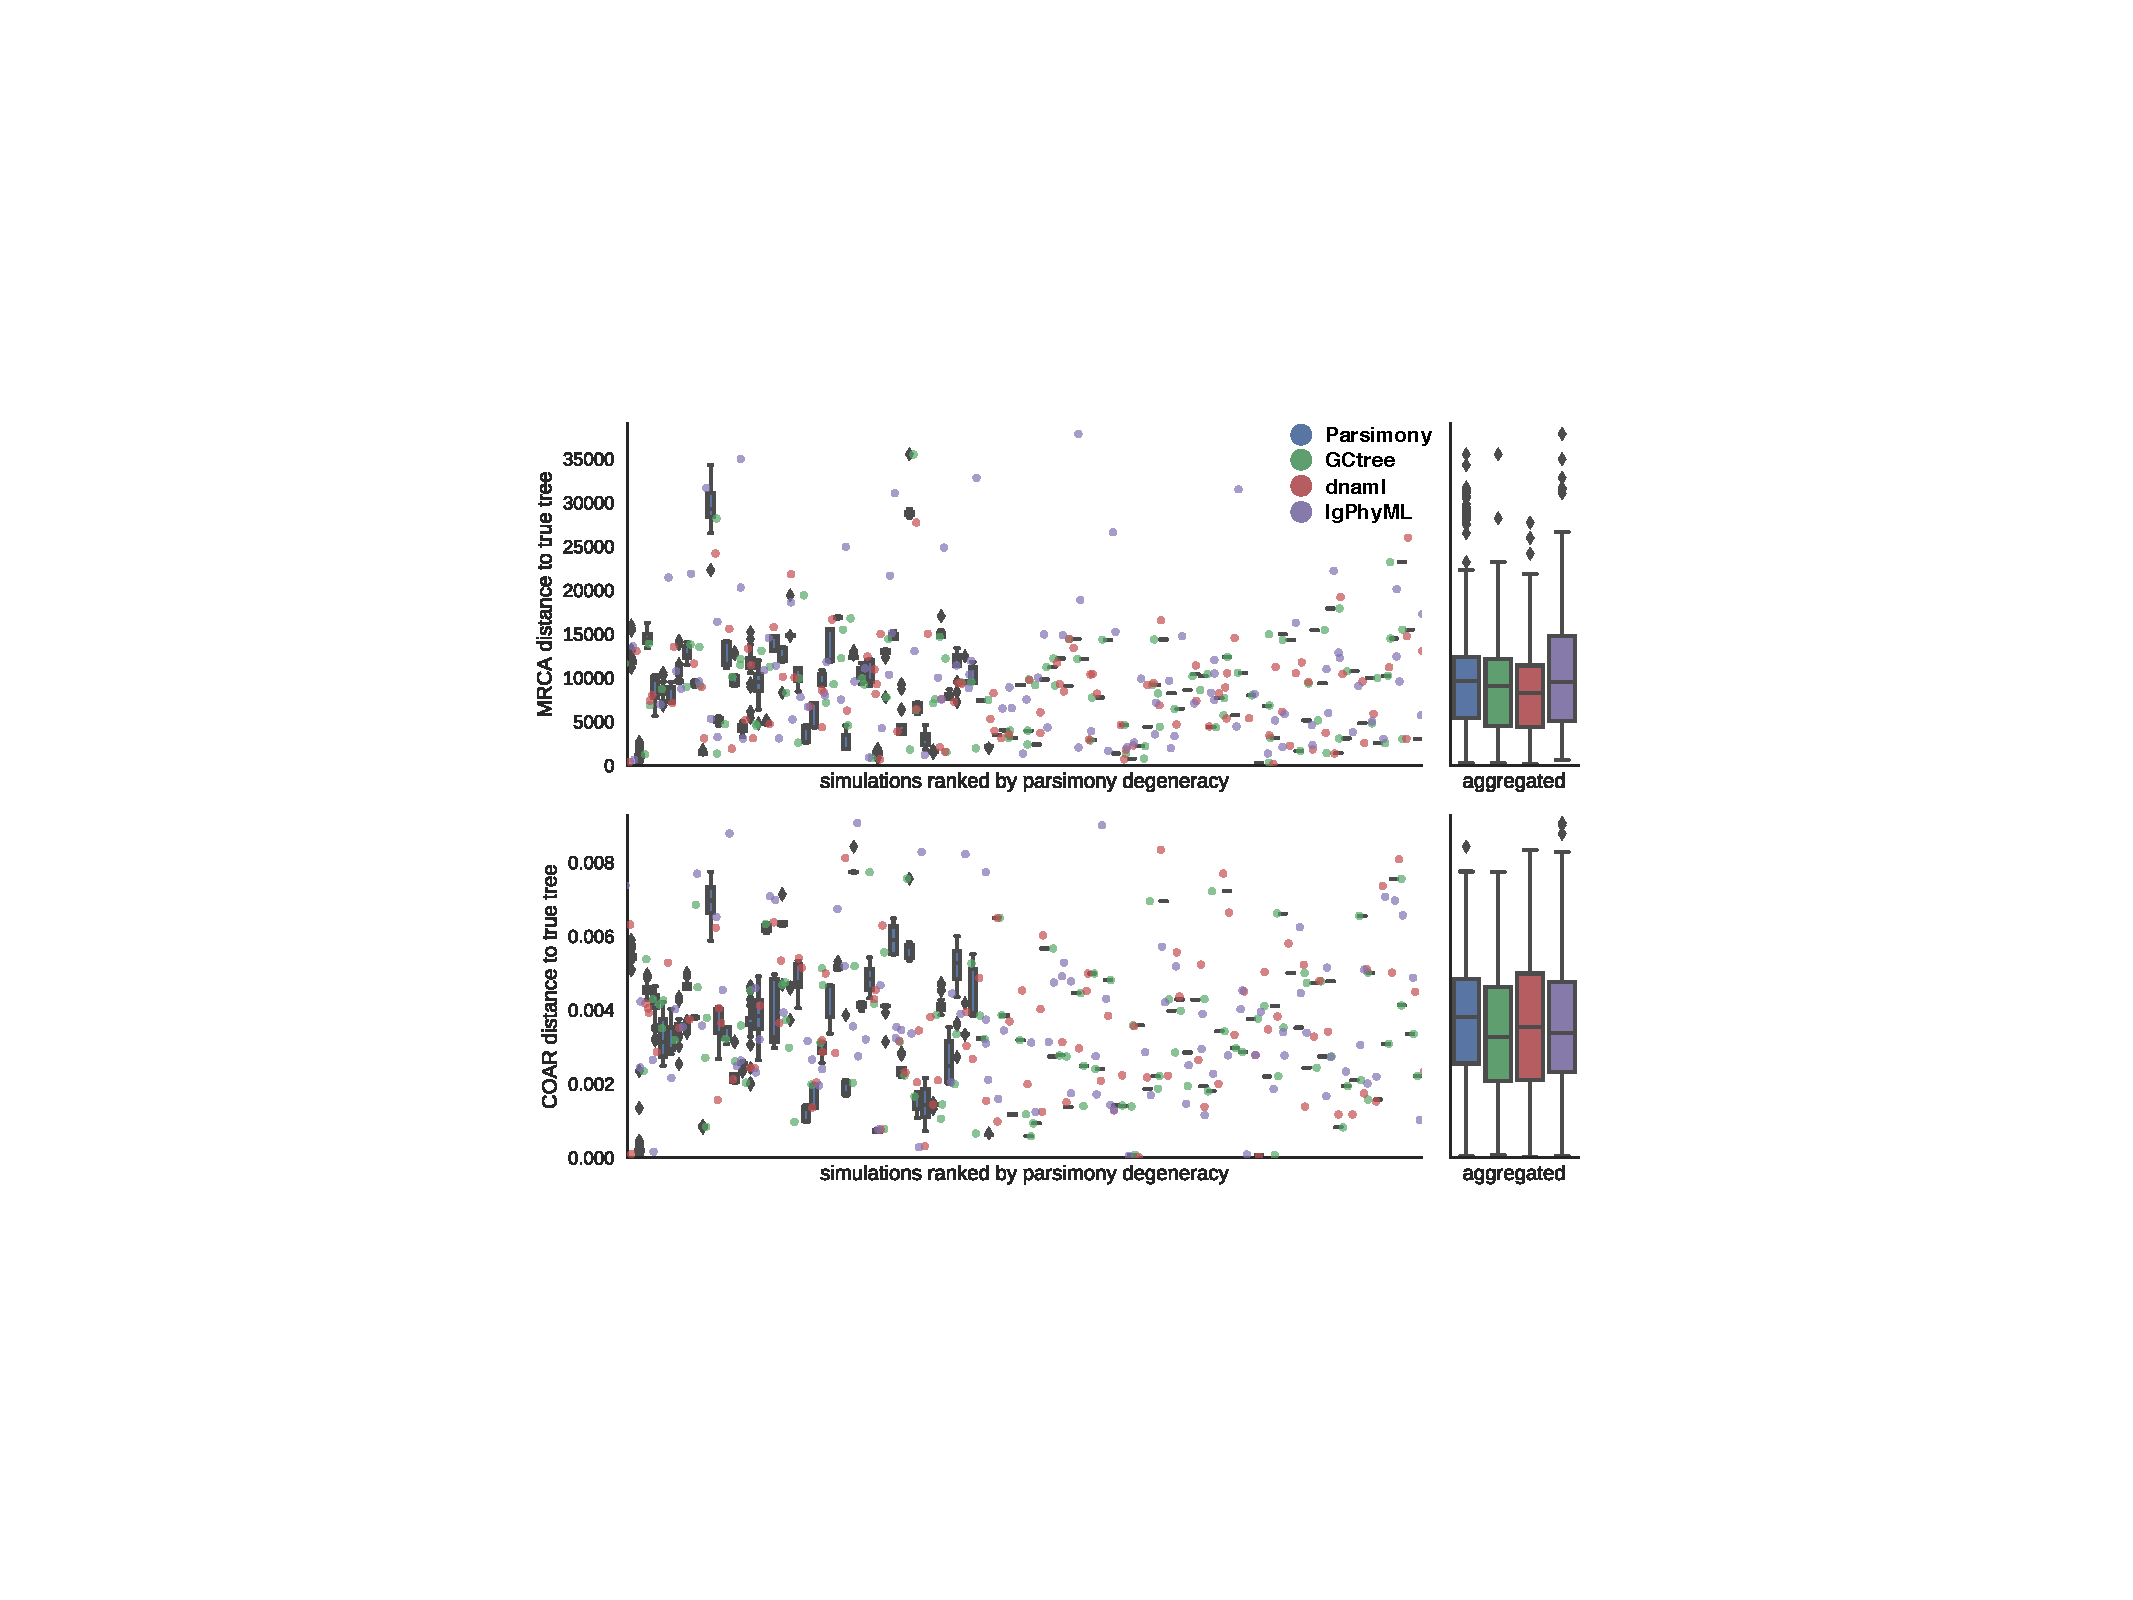
\includegraphics[width=0.9\textwidth]{figures/Laura-affsim_valid.pdf}
    \caption{
        \label{fig:Laura-affsim_valid}
        Simulation with 100 repeats of the affinity simulation.
        Each simulation is plotted in a single column ranked according to the number of equally parsimonious trees for the simulation.
        The ensemble of equally parsimonious trees are shown as a box plot while the other methods are plotted as jittered dots.
        On the right the aggregated result is shown.
    }
\end{figure}






\section{Discussion and conclusion}
Tree topology is not the biggest concern in this validation because often the topology is not a very important objective by itself.
It is the reconstructed sequences and the order of these, the selection pressure etc. that is most important.
These objectives then tend to be correlated with correct tree topology, but that does not necessarily need to be true, and therefore the main objective is to validate ASR and let the tree topology follow as a consequence of improving the ASR.

The presented COAR metric is a suitable objective for ASR since it is robust to irrelevant errors in tree topology and directly interpretable as the expected per site error of sequences in a reconstructed lineage.
The simulation study we present show that, regardless of the inference method used, the reconstruction of sequences along an ancestral lineage is robust and only rarely accumulate errors.
In a worst-case scenario there is an expected one nucleotide error per reconstructed sequence in a reconstructed lineage, based on affinity simulation with 4-8 sequences (including the a priori know root and leaf) in a lineage, see b) in figure \ref{fig:Laura-affsim_runstat} appendix B.

Simulating under a neutral branching process is not realistic compared to the fast and stringent selection process which is undertaken in the GC reaction.
The simulation with added affinity selection addresses this issue and challenges the inference methods with both epistasis and homoplasy.
Therefore it is not surprising to see that inference on affinity simulations obtain higher COAR values than neutral simulation under comparable conditions.
What is surprising is that all inference methods seems to be equally effected by the imposed affinity selection.
We would have expected a codon based model like IgPhyML to have a an advantage compared to the nucleotide based models because affinity selection is strictly on protein level, and hence there is a preference for synonymous over non-synonymous mutations that is incorporated in the model parameters of a codon model but not in a nucleotide model.
IgPhyML should also have an advantage over the other methods due to its incorporation of AID hot/cold spot motif in its model.
Although IgPhyML is marginalizing over motifs that span multiple codons, to achieve site independence, it should still capture some of the signal from mutational context bias.
Again this does not seem to improve the inference by IgPhyML over the other method.

Looking at typical trees simulated from both the neutral -and affinity selected process (see trees in appendix B) it look like trees are relatively shallow i.e. the number of internal nodes from the leaf to the root is small.
This of course makes it easier to get a low COAR score because there are only few states to reconstruct.
In the affinity model trees are simulated over a long time range but still appear shallow because cells with low affinity are lost during maturation.
On a tree this memory loss of lower affinity variants will show as a tree with a long trunk extending from the root to a bushy canopy, similar to observations made by Yaari et al. \cite{yaari2015mutation} (visualized in b) in figure \ref{fig:Laura-affsim_runstat} in appendix B).
This trait could explain why is there is no apparent benefit of integrating AID motifs into an inference algorithm like IgPhyML.

The overall performance of all the evaluated inference methods is very similar.
There is a consistent ranking that puts GCtree first, dnaml and IgPhyML second and sets Parsimony last, but it must be stressed that the difference is very small and that the performance can be regarded as practically equivalent.
GCtree that stands out as the most consistently better performing algorithm is also dependent on the genotype abundance which is not readily available for most BCR data.
Abundance data could potentially be extracted from standard HTS data but because of sequencing errors and primer biases these abundances are not reliable.
With the introduction of UMIs this problem is getting addressed and it is expected that in most future datasets that the abundance information will be more reliable, giving the opportunity to integrate abundance data in methods such as GCtree to direct phylogenetic inference.




\section{Conclusion}
The problem of inferring BCR phylogenies appears to be insensitive to the method used on the simulation regimes tested.
With a significant improvement of GCtree inference we suggest that this is used when reliable abundance information exists.
Otherwise the methods tested are practically equivalent suggesting that users should care mostly about which tool provide the most convenient solution to inferring their BCR phylogeny.
It remains to be tested whether different sampling conditions, such as time series sampling, will alter the results.
Likewise it is undetermined if joint reconstruction will do any improvement over marginal reconstruction.


